\chapter{Aspetos da Implementação} \label{cap:implementacao}
Esta secção tem como propósito clarificar e justificar as várias decisões que tomámos no desenvolvimento dos vários módulos do projeto. \\
Na secção \ref{sec:ecra} iremos apresentar os vários ecrãs da aplicação móvel desenvolvida.

\section{Ecrãs da Aplicação Móvel} \label{sec:ecra}
Nesta secção apresentamos os vários ecrãs ou páginas da aplicação móvel.\\
Na figura \ref{fig:1} está a página de \textit{log-in}.

\begin{figure}[ht!]
\centering
\resizebox{50mm}{!}{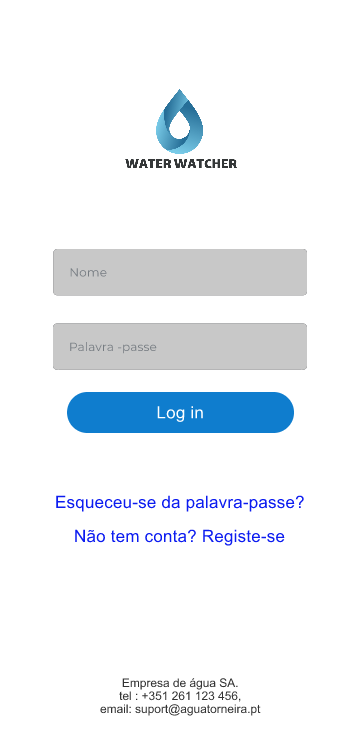
\includegraphics{diagramas/app/1.png}}
\caption{Página de log-in.}
\label{fig:1}
\end{figure}

Nesta página é possível o utilizador inserir as suas credenciais para entrar na aplicação. Também é possível registar uma nova conta ou recuperar o acesso a uma conta. Esta página apresenta também os contactos da empresa.\\
Depois de efetuado o \textit{log-in}, o utilizador é encaminhado para a página principal, apresentada na figura \ref{fig:2}.

\begin{figure}[ht!]
\centering
\resizebox{50mm}{!}{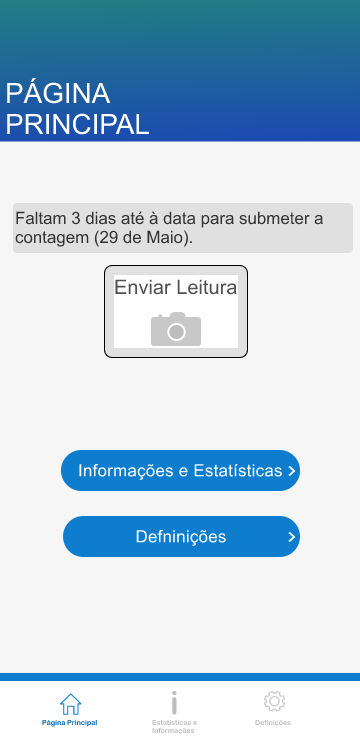
\includegraphics{diagramas/app/2.png}}
\caption{Página principal}
\label{fig:2}
\end{figure}

É neste ecrã que o utilizador poderá enviar a fotografia do contador no dia designado. \\
A partir deste ecrã, tem também a possibilidade de aceder às informações e estatísticas presentes no ecrã representado na figura \ref{fig:3}. 

\vspace{8.5cm}

\begin{figure}[ht!]
\centering
\resizebox{50mm}{!}{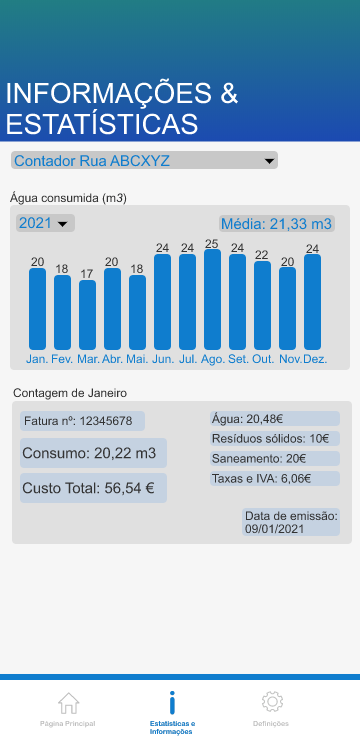
\includegraphics{diagramas/app/3.png}}
\caption{Página de informações e estatísticas}
\label{fig:3}
\end{figure}

A página de informações e estatísticas é onde estão disponíveis vários dados referentes ao serviço e detalhes das faturas do utilizador.\\ Por fim, é possível aceder ao ecrã de definições representado na figura \ref{fig:4}.

\vspace{20cm}

\begin{figure}[ht!]
\centering
\resizebox{50mm}{!}{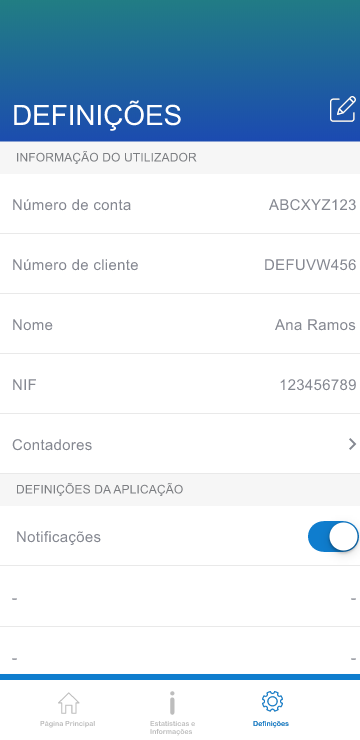
\includegraphics{diagramas/app/4.png}}
\caption{Página de definições.}
\label{fig:4}
\end{figure}

Nesta página, o utilizador pode ver e editar as suas informações e preferências da aplicação. Mais concretamente, também é possível gerir os contadores associados à sua conta, no ecrã da figura \ref{fig:5}.

\begin{figure}[ht!]
\centering
\resizebox{50mm}{!}{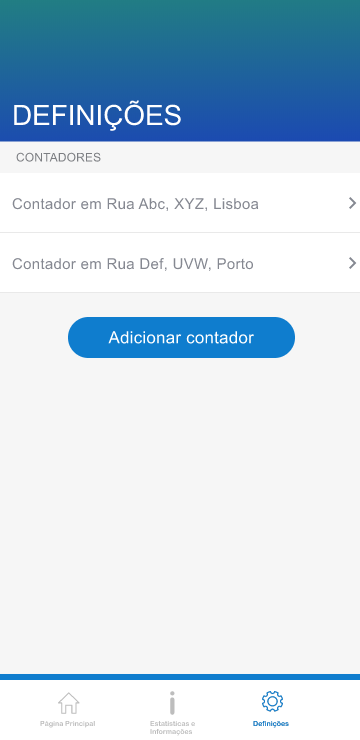
\includegraphics{diagramas/app/5.png}}
\caption{Página de definições relacionadas com os contadores.}
\label{fig:5}
\end{figure}












